让我们通过一个使用noexcept关键字的小示例来开始这个主题。\par

\hspace*{\fill} \par %插入空行
\textbf{7.1.1 无noexcept的移动构造函数}

考虑下面的类,引入了一个带有string成员的类型,并实现了一个复制和一个移动构造函数:\par

{\color{red}{basics/person.hpp}}\par

\begin{lstlisting}[caption={}]
#include <string>
#include <iostream>

class Person {
	private:
	std::string name;
	public:
	Person(const char* n)
	: name{n} {
	}

	std::string getName() const {
		return name;
	}

	// print out when we copy or move:
	Person(const Person& p)
	: name{p.name} {
		std::cout << "COPY " << name << '\n';
	}
	Person(Person&& p)
	: name{std::move(p.name)} {
		std::cout << "MOVE " << name << '\n';
	}
	...
};
\end{lstlisting}

现在我们创建并初始化一个Person的vector,并插入一个Person:\par

{\color{red}{basics/person.cpp}}\par

\begin{lstlisting}[caption={}]
#include "person.hpp"
#include <iostream>
#include <vector>

int main()
{
	std::vector<Person> coll{"Wolfgang Amadeus Mozart",
		"Johann Sebastian Bach",
		"Ludwig van Beethoven"};
	std::cout << "capacity: " << coll.capacity() << '\n';
	coll.push_back("Pjotr Iljitsch Tschaikowski");
}
\end{lstlisting}

程序输出如下:\par

\begin{tcolorbox}[colback=white,colframe=black]
COPY Wolfgang Amadeus Mozart \\
COPY Johann Sebastian Bach \\
COPY Ludwig van Beethoven \\
capacity: 3 \\
MOVE Pjotr Iljitsch Tschaikowski \\
COPY Wolfgang Amadeus Mozart \\
COPY Johann Sebastian Bach \\
COPY Ludwig van Beethoven
\end{tcolorbox}

首先,将初始值复制到vector中(因为容器的std::initializer\_list<>构造函数按值接受传递的参数)。因此,vector通常为三个元素分配内存(在图中,我使用了字符串值的快捷方式):\par

\begin{center}
	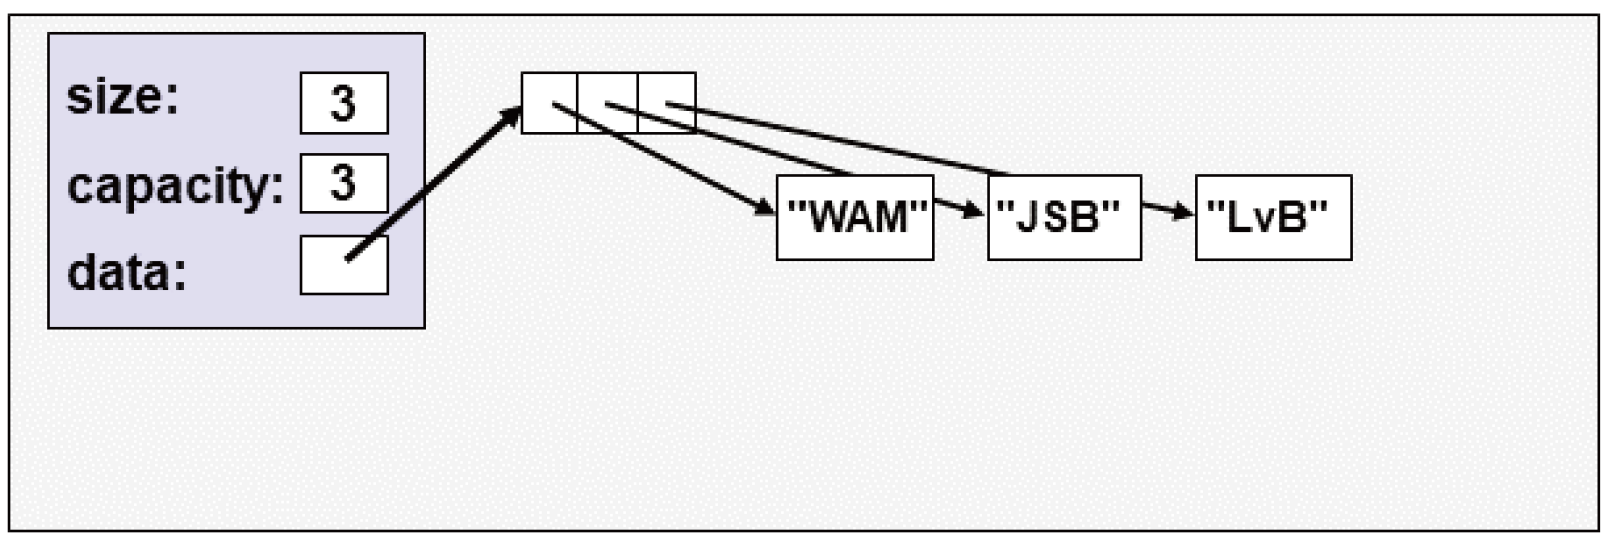
\includegraphics[width=1.0\textwidth]{content/1/chapter7/images/1}
\end{center}

接下来会发生什么:我们用push\_back()插入第四个元素,结果如下:\par

\begin{itemize}
	\item 因为vector在内部需要更多内存,所以它分配新的内存(比如,6个元素),移动第四个字符串(创建一个临时的Person并使用push\_back()方法将其移动到vector中),但也将现有的元素复制到新内存中:\par
	\begin{center}
		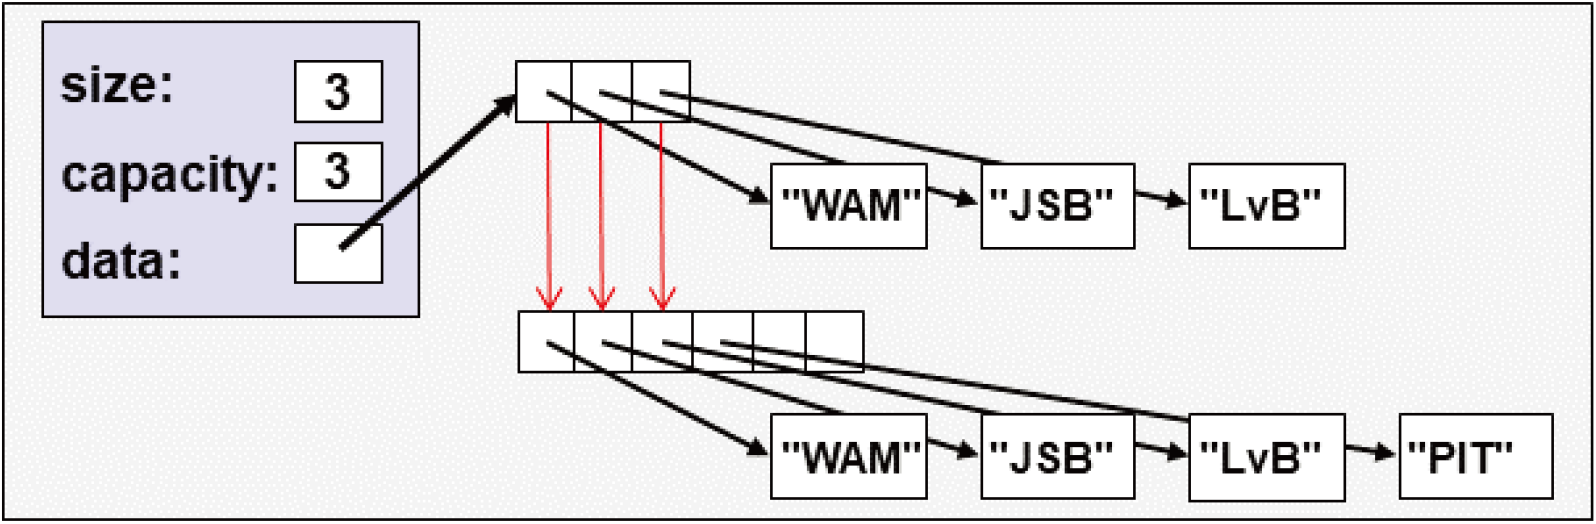
\includegraphics[width=1.0\textwidth]{content/1/chapter7/images/2}
	\end{center}
	\item 这个操作结束时,vector销毁旧的元素,释放这些元素的旧内存,并更新其成员:\par
	\begin{center}
		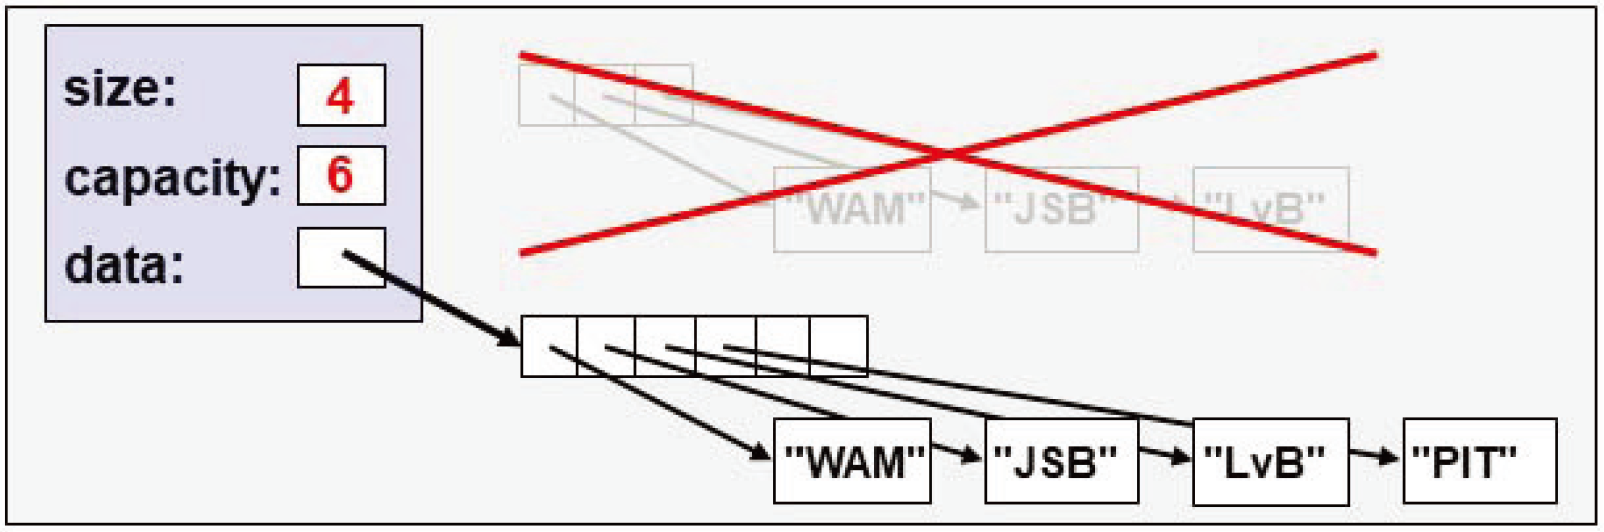
\includegraphics[width=1.0\textwidth]{content/1/chapter7/images/3}
	\end{center}
\end{itemize}

问题是,为什么vector不使用移动构造函数,将元素从旧内存移动到新内存呢?\par

\hspace*{\fill} \par %插入空行
\textbf{强异常安全保证}

vector的重新分配不使用移动语义的原因是,push\_back()提供了强异常处理保证:当在vector的重新分配过程中抛出异常时,C++标准库保证将vector回滚到之前的状态。也就是说,push\_back()提供了一种事务保证:要么成功,要么无效。\par

C++标准能够在C++98和C++03中提供这种保证,因为C++只能复制元素。如果在复制元素时出现错误,源对象仍然可用。处理异常的内部代码只是销毁创建的副本,并释放新的内存,使vector返回到之前的状态(C++标准库要求析构函数不抛出异常;否则,无法回滚)。\par

重新分配是使用移动语义的完美位置,因为我们将元素从一个位置移动到另一个位置。因此,在C++11中我们希望在这里使用移动语义。但是,如果在重新分配期间抛出异常,我们可能无法回滚。新内存中的元素已经窃取了旧内存中元素的值。因此,只是销毁新的元素是不够的,还得把他们移回去。但我们怎么知道把它们移回就不会失败呢?\par

你可能会说一个移动构造函数永远不抛出异常。这可能是正确的字符串(因为我们只是移动值和指针),而是需要对象在一个有效的状态,这种状态可能需要额外的内存,所以当额外内存有问题时会丢弃状态信息(例如,基于节点的容器Visual c++实现方式)。\par

我们也不能放弃,因为程序可能已经使用这个特性来避免创建向量的备份,而丢失数据可能是(安全)关键的。不再支持push\_back()对于使用C++11来说将是个噩梦。\par

最后,只有当元素类型的移动构造函数保证不会抛出异常时,才在重新分配时使用移动语义。\par

\hspace*{\fill} \par %插入空行
\textbf{7.1.2 使用noexcept的移动构造函数}

因此,当我们保证Person类的移动构造函数永远不会抛出异常时,我们的示例程序就改变了它的行为:\par

{\color{red}{basics/personmove.hpp}}\par

\begin{lstlisting}[caption={}]
#include <string>
#include <iostream>

class Person {
	private:
	std::string name;
	public:
	Person(const char* n)
	: name{n} {
	}
	std::string getName() const {
		return name;
	}

	// print out when we copy or move:
	Person(const Person& p)
	: name{p.name} {
		std::cout << "COPY " << name << '\n';
	}
	Person(Person&& p) noexcept // guarantee not to throw
	: name{std::move(p.name)} {
		std::cout << "MOVE " << name << '\n';
	}
	...
};
\end{lstlisting}

如果像以前一样使用Persons:\par

{\color{red}{basics/personmove.cpp}}\par

\begin{lstlisting}[caption={}]
#include "personmove.hpp"
#include <iostream>
#include <vector>

int main()
{
	std::vector<Person> coll{"Wolfgang Amadeus Mozart",
		"Johann Sebastian Bach",
		"Ludwig van Beethoven"};
	std::cout << "capacity: " << coll.capacity() << '\n';
	coll.push_back("Pjotr Iljitsch Tschaikowski");
}
\end{lstlisting}

我们得到以下输出:\par

\begin{tcolorbox}[colback=white,colframe=black]
COPY Wolfgang Amadeus Mozart \\ 
COPY Johann Sebastian Bach \\
COPY Ludwig van Beethoven \\
capacity: 3 \\
MOVE Pjotr Iljitsch Tschaikowski \\
MOVE Wolfgang Amadeus Mozart \\
MOVE Johann Sebastian Bach \\
MOVE Ludwig van Beethoven
\end{tcolorbox}

同样,首先将初始值复制到vector中\par

\begin{center}
	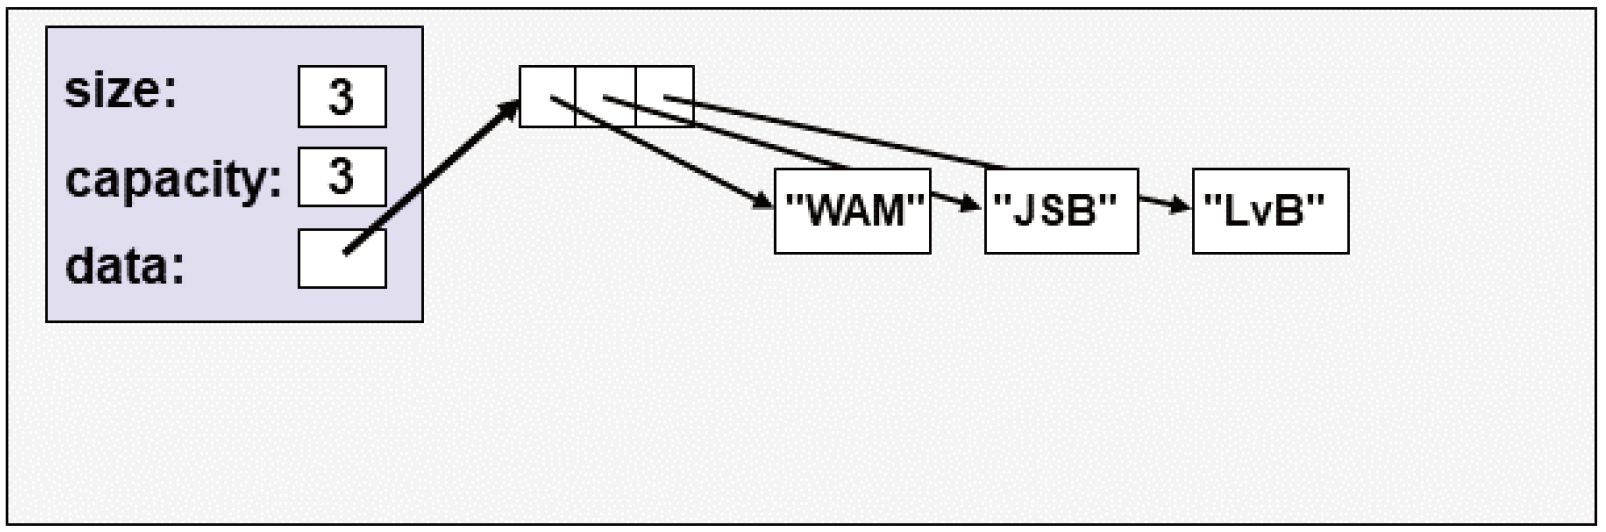
\includegraphics[width=1.0\textwidth]{content/1/chapter7/images/4}
\end{center}

然而,随着输出的最后三行可视化,vector现在使用移动构造函数将元素移动到新的重新分配的内存中:\par

\begin{center}
	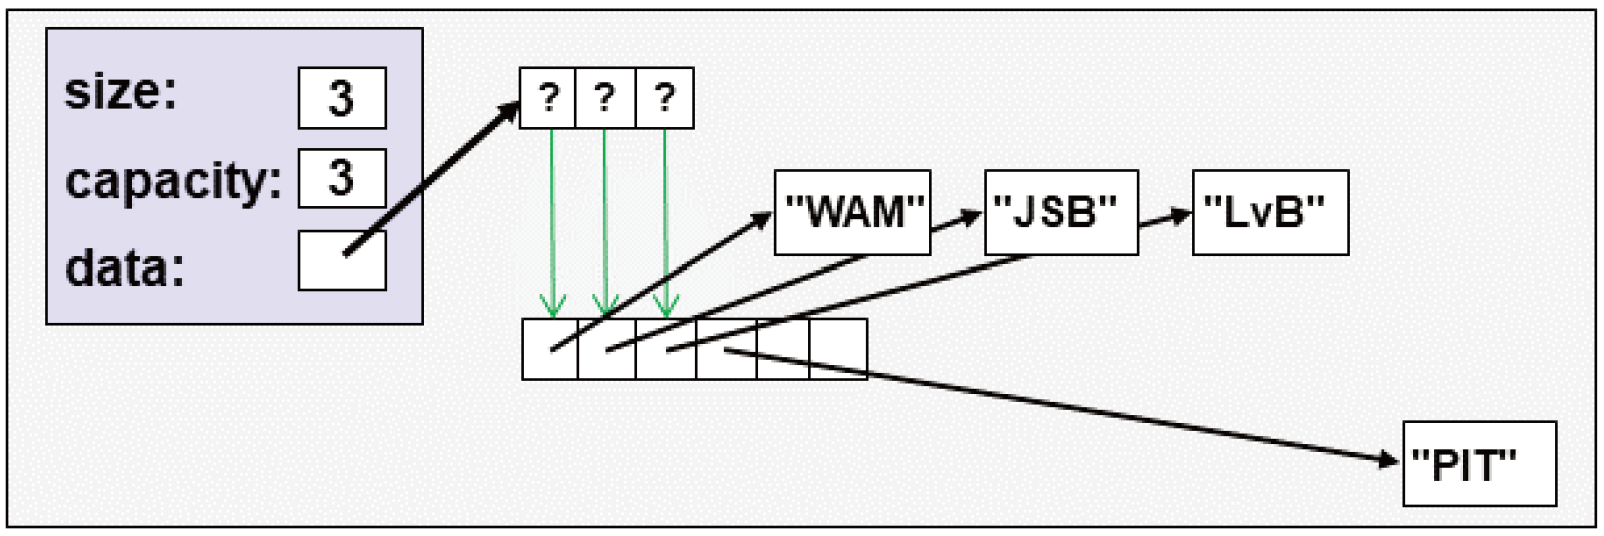
\includegraphics[width=1.0\textwidth]{content/1/chapter7/images/5}
\end{center}

最后,vector只需要释放旧内存并更新其成员:\par

\begin{center}
	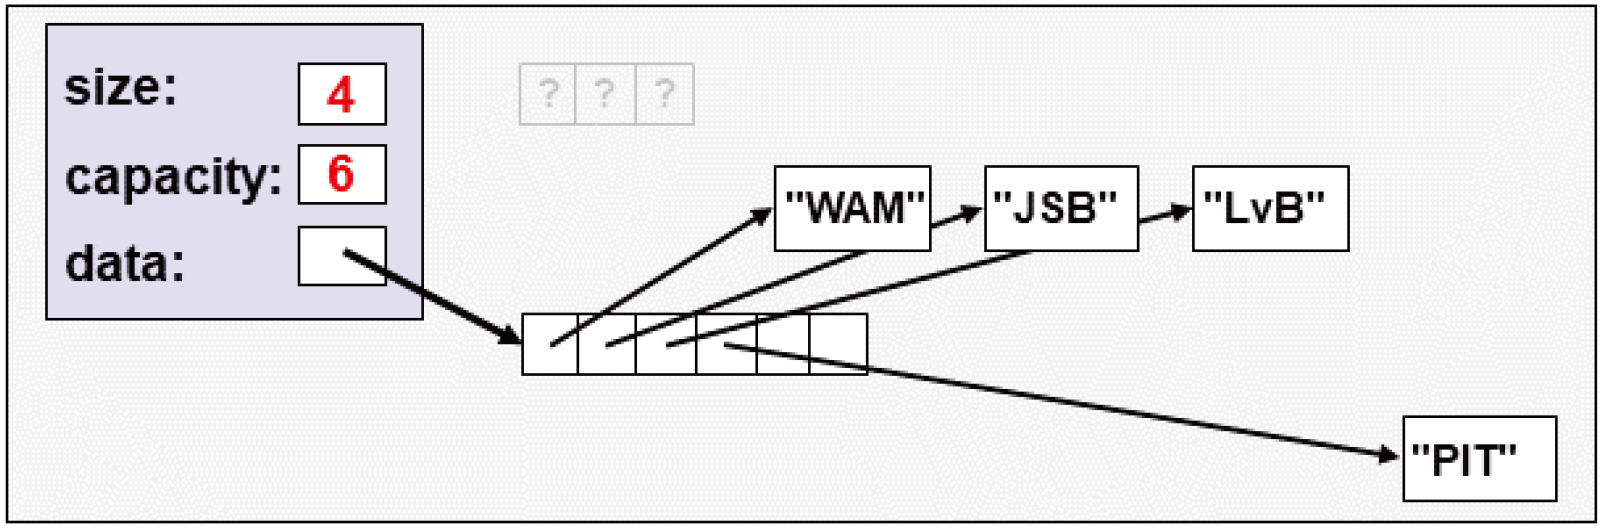
\includegraphics[width=1.0\textwidth]{content/1/chapter7/images/6}
\end{center}

\hspace*{\fill} \par %插入空行
\textbf{具有条件的noexcept声明}

然而,是否可以将移动构造函数标记为noexcept?我们移动了name(一个std::string),并向标准输出流写入一些内容。如果我们在那里抛出异常,我们就违反了无异常的保证。在这种情况下,程序在运行时将调用std::terminate(),后者通常调用std::abort()来发出程序异常结束的信号(通常会出现core dump)。\par

因此,如果string成员和输出操作不抛出异常,则应该保证不抛出异常。引入noexcept关键字是因为可以使用它来指定不抛出的条件保证。它看起来是这样的({\color{red}{basics/personcond.hpp}}为完整的例子):\par

\begin{lstlisting}[caption={}]
class Person {
	private:
		std::string name;
	public:
		...
		Person(Person&& p)
		noexcept(std::is_nothrow_move_constructible_v<std::string>
		&& noexcept(std::cout << name))
		: name{std::move(p.name)} {
			std::cout << "MOVE " << name << '\n';
		}
		...
\end{lstlisting}

使用noexcept(…),保证在括号内的编译时表达式为真时不会抛出异常。这种情况下,我们需要两样东西来保证:\par

\begin{itemize}
	\item 对于std::is\_nothrow\_move\_constructible\_v<std::string>(在C++20之前,必须使用std::is\_nothrow\_move\_constructible<std::string>::value),我们使用标准类型特征(type)来告诉我们std::string的移动构造函数是否保证不抛出异常。
	\item 对于noexcept(std::cout << name),我们查询来了对名称的输出表达式的调用是否保证不抛出异常。这里,我们使用noexcept作为操作符,它告诉我们是否所有执行传递的表达式的相应操作都保证不会抛出异常。
\end{itemize}

通过此声明,重新分配将再次使用复制构造函数。字符串的移动构造函数不保证抛出异常,但输出操作符不保证抛出异常。然而,移动构造函数通常不输出任何内容。因此,通常当成员不抛出异常时,可以为整个移动构造函数提供不抛出异常的保证。\par

好消息是,如果没有自己实现移动构造函数,编译器将为你提供noexcept保证。对于所有成员都保证不抛出移动构造函数的类,生成的或默认的移动构造函数将作为整体提供保证。\par

考虑下面的声明:\par

{\color{red}{basics/persondefault.hpp}}\par

\begin{lstlisting}[caption={}]
#include <string>
#include <iostream>

class Person {
	private:
	std::string name;
	public:
	Person(const char* n)
	: name{n} {
	}

	std::string getName() const {
		return name;
	}

	// print out when we copy:
	Person(const Person& p)
	: name{p.name} {
		std::cout << "COPY " << name << '\n';
	}
	// force default generated move constructor:
	Person(Person&& p) = default;
	...
};
\end{lstlisting}

这种情况下,应该生成默认的移动构造函数:\par

\begin{lstlisting}[caption={}]
class Person {
	...
	// force default generated move constructor:
	Person(Person&& p) = default;
	...
};
\end{lstlisting}

这意味着只有在复制时才打印。当使用生成的移动构造函数时,我们只看到没有执行复制。\par

现在让我们用常用的程序在末尾打印一些Persons:\par

{\color{red}{basics/persondefault.cpp}}\par

\begin{lstlisting}[caption={}]
#include "persondefault.hpp"
#include <iostream>
#include <vector>

int main()
{
	std::vector<Person> coll{"Wolfgang Amadeus Mozart",
		"Johann Sebastian Bach",
		"Ludwig van Beethoven"};
	std::cout << "capacity: " << coll.capacity() << '\n';
	coll.push_back("Pjotr Iljitsch Tschaikowski");
	
	std::cout << "name of coll[0]: " << coll[0].getName() << '\n';
}
\end{lstlisting}

我们会得到以下输出:\par

\begin{tcolorbox}[colback=white,colframe=black]
COPY Wolfgang Amadeus Mozart \\
COPY Johann Sebastian Bach \\
COPY Ludwig van Beethoven \\
capacity: 3 \\
name of coll[0]: Wolfgang Amadeus Mozart
\end{tcolorbox}

我们只看到初始化器列表中元素的副本。对于其他任何的操作,包括重新分配,都使用默认的移动构造函数。正如我们所看到的,在重新分配的内存中,第一人名是正确的。\par

如果不指定任何成员函数,则具有相同的行为。这意味着:\par

\begin{itemize}
	\item 如果实现了一个移动构造函数,应该声明它是否以及何时保证不会抛出异常。
	\item 如果不需要实现移动构造函数,根本不需要指定任何东西。
\end{itemize}

如果一个类的性能或该类的重新分配对象很重要,你可能还想在编译时再次检查类的移动构造函数是否保证不会抛出异常:\par

\begin{lstlisting}[caption={}]
static_assert(std::is_nothrow_move_constructible_v<Person>);
\end{lstlisting}

或升级到C++17:\par

\begin{lstlisting}[caption={}]
static_assert(std::is_nothrow_move_constructible<Person>::value, "");
\end{lstlisting}

\hspace*{\fill} \par %插入空行
\textbf{7.1.3 值得使用noexcept吗?}

您可能想知道用或多或少的noexcept表达式声明移动构造函数是否值得使用。Howard Hinnant用一个简单的程序演示了这种效果(本书稍微改编):\par

{\color{red}{basics/movenoexcept.cpp}}\par

\begin{lstlisting}[caption={}]
#include <iostream>
#include <string>
#include <vector>
#include <chrono>

// string wrapper with move constructor:
struct Str
{
	std::string val;
	// ensure each string has 100 characters:
	Str()
	: val(100, 'a') { // don’t use braces here
	}

	// enable copying:
	Str(const Str&) = default;
	
	// enable moving (with and without noexcept):
	Str (Str&& s) NOEXCEPT
	: val{std::move(s.val)} {
	}
};

int main()
{
	// create vector of 1 Million wrapped strings:
	std::vector<Str> coll;
	coll.resize(1000000);
	
	// measure time to reallocate memory for all elements:
	auto t0 = std::chrono::steady_clock::now();
	coll.reserve(coll.capacity() + 1);
	auto t1 = std::chrono::steady_clock::now();
	
	std::chrono::duration<double, std::milli> d{t1 - t0};
	std::cout << d.count() << "ms\n";
}
\end{lstlisting}

我们提供了一个类来包装长度有效的字符串(以避免小字符串优化)。注意,必须用圆括号初始化,因为大括号会将100解释为值为100的初始字符。\par

在类中,我们用NOEXCEPT标记移动构造函数,预处理程序可以用nothing或noexcept (例如,用-DNOEXCEPT= NOEXCEPT编译)来替换它。然后,我们再看看重新分配vector中的100万个对象需要多长时间。\par

在几乎所有平台上,声明onexcept的移动构造函数会使重新分配速度提高10倍(确保激活了显著的优化级别)。也就是说,重新分配(通常通过插入新元素强制执行)可能需要20毫秒,而不是200毫秒。这意味着减少了180毫秒,我们不能使用任何其他向量,这对于性能来说是一个巨大的收益。\par





